\subsection{Uso del triac y diac}
    Como en el presente trabajo práctico (TP), se utiliza un circuito de
    disparo compuesto con un triac y un diac, se explica brevemente
    de que trata cada dispositivo y como se forma el circuito de la placa
    propia del TP.
    
    \subsubsection{Diac}
        El diac es un dispositivo semiconductor, que posee cuatro capas de semiconductores  
        y dos terminales de conexión, como se observa en la Figura \ref{fig:EstrucDiac}. 
        Tiene la particularidad de poder circular corriente en ambos sentidos cuando es 
        activado. Dicha activación en el diac, ocurre cuando se alcanza el voltaje de ruptura 
        \(V_{BO}\) en cualquiera de los dos sentidos, y se apaga cuando la corriente se 
        reduce por debajo del valor de retención mencionado. 
        La curva del dispositivo se observa en la Figura \ref{fig:CurvaDiac}. 

        \begin{figure}[H]
            \centering
            \begin{subfigure}[ht]{0.48\textwidth}
              \frame{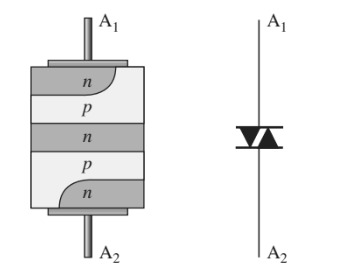
\includegraphics[width=\textwidth]{Imagenes/MarcoTeorico/TRIACyDIAC/DIAC2.jpeg}}
              \caption{Estructura y símbolo del diac.}
              \label{fig:EstrucDiac}
            \end{subfigure}
            \hfill 
            \begin{subfigure}[ht]{0.48\textwidth}
              \frame{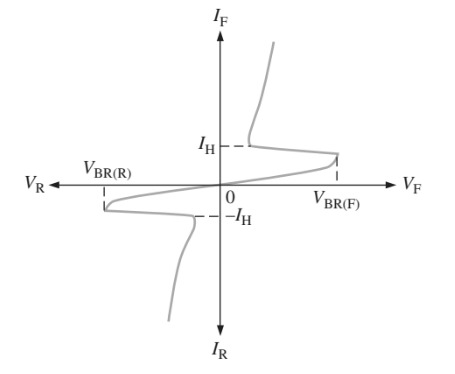
\includegraphics[width=\textwidth]{Imagenes/MarcoTeorico/TRIACyDIAC/curvaDIAC.jpeg}}
              \caption{Curva de trabajo del diac.}
              \label{fig:CurvaDiac}
            \end{subfigure}
            \caption{Características del diac.}
        \end{figure}

    \subsubsection{Triac}
        
        El triac es como un diac pero con un terminal de compuerta G (\textit{gate}), 
        el cual le permite ser disparado por un pulso de corriente en dicha terminal.
        A diferencia del diac, no requiere de un voltaje de ruptura para iniciar 
        la conducción. 
        Este dispositivo es capaz, también como el diac, de conducir corriente en ambos
        sentidos según la polaridad de voltaje que tenga entre sus bornes. La construcción, 
        el símbolo y la curva de trabajo del triac se observan en la 
       Figura \ref{fig:DatosTriac}.


        \begin{figure}[H]
            \centering
            \begin{subfigure}[ht]{0.48\textwidth}
              \frame{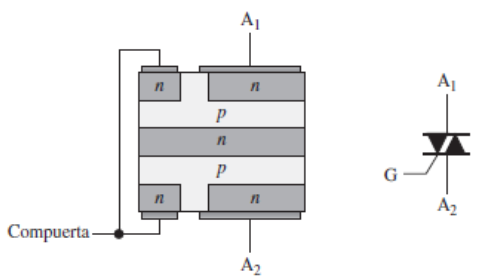
\includegraphics[width=\textwidth]{Imagenes/MarcoTeorico/TRIACyDIAC/simboloTRIAC.png}}
              \caption{Estructura y símbolo del triac.}
              \label{fig:EstrucTriac}
            \end{subfigure}
            \hfill 
            \begin{subfigure}[ht]{0.48\textwidth}
              \frame{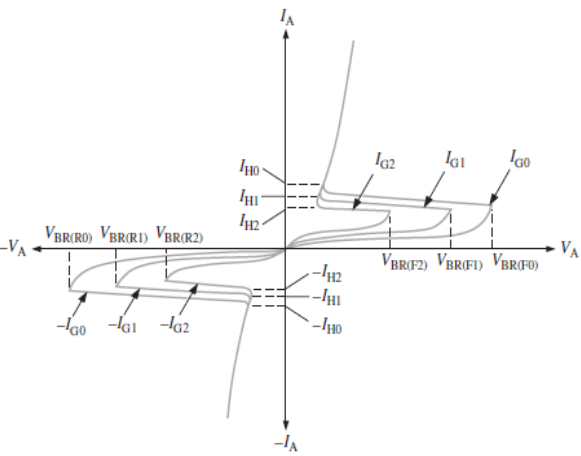
\includegraphics[width=\textwidth]{Imagenes/MarcoTeorico/TRIACyDIAC/curvaTRIAC.png}}
              \caption{Curva de trabajo del triac.}
              \label{fig:CurvaTriac}
            \end{subfigure}  
            \caption{Características del triac.}
            \label{fig:DatosTriac}
        \end{figure}

    \subsubsection{Circuito de disparo con triac y diac}
        
        Para este trabajo práctico se utiliza el siguiente circuito de disparo 
        de triac con diac (\textit{dimmer}) que se observa en la Figura 
        \ref{fig:CircuitoTriacDiac}

        \begin{figure}[H]
            \centering
            \frame{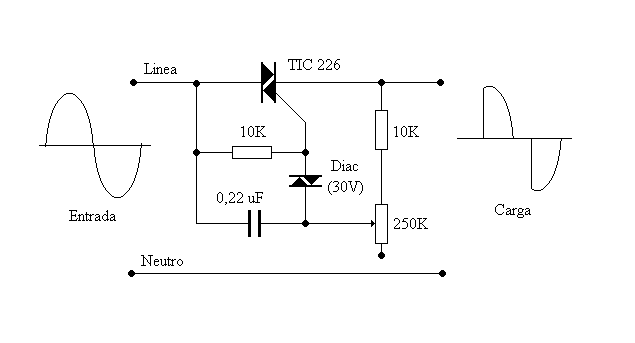
\includegraphics[width=0.45\textwidth]{Imagenes/MarcoTeorico/TRIACyDIAC/Esquema_Circuito_Angulo_Disparo.png}}
            \caption{Circuito dimmer con triac y diac.}
            \label{fig:CircuitoTriacDiac}
          \end{figure}

        El potenciómetro de 250~\(K\Omega\), lo que hace es regular el tiempo de carga del condensador 
        de 0.22~\(\mu F\), el cual es el encargado de entregar la tensión de ruptura (30~V) 
        para que el diac conduzca. Una vez que el diac conduce, deja pasar una corriente 
        la cual activa al triac a través de su terminal G. Este último dejará de conducir 
        cuando la corriente sea menor al valor de retención (aproximadamente cuando la 
        tensión de entrada cruce por cero).
        Para que vuelva a conducir en el semiciclo negativo, el capacitor es cargado con
        polarización inversa a la anterior, y dispara el diac cuando llega a la tensión 
        de ruptura nuevamente. De esta manera, se genera un nuevo pulso en el gate del 
        triac y el mismo conducirá en el otro sentido de la corriente.

        Como se observa en el esquemático entre el terminal G del triac y un ánodo del diac, 
        se tiene una resistencia limitadora de corriente para el terminal G de 10~\(K\Omega\).
        Además, dicha resistencia permite cerrar el circuito del capacitor para descargarlo.

        Por último, la otra resistencia de 10~\(K\Omega\) y el potenciómetro 
        (conectados en serie) permiten variar el tiempo de carga del capacitor, partiendo 
        de un mínimo de \(2.2~ms\). Dichas resistencias en serie también cumplen la 
        función de limitar la corriente para el circuito de disparo. 
